%%==================================================
%% chapter03.tex for TJU Master Thesis
%% Encoding: UTF-8
%%==================================================

\chapter{纤维编织加强软管组件拉伸实验}
\section{引~言}

很早就有学者用拉伸实验开始研究纤维编织加强层。\citeauthor{brunnschweiler19545}\cite{brunnschweiler19545}用拉伸试验机对不同编织角的编织层进行了测试。发现使得编织结构失效的拉伸量,至少是编织层所用纤维失效拉伸量的$ 150\% $以上。单位面积内的股数与编织层失效拉伸量正相关,同样也与初始编织角相关。\citeauthor{Harte20001259}\cite{Harte20001259,Harte2000259}研究了符合材料编织层拉伸时的力学行为和颈缩现象。发现编织结构能非常有效的吸收能量,在拉伸过程中,编织层发生较大的拉伸应变时,纤维上的拉伸应变是恒定值。\citeauthor{Hachemi2011}\cite{Hachemi2011}采用了拉伸实验作为检验其模型的手段。


也有学者对拉伸试验的实验测试技术进行了研究和提升,\citeauthor{Leung2013}\cite{Leung2013}
采用了双镜头显微摄像仪(stereomicroscope)以及数字图像修正技术(digital image correlation,DIC)研究了拉伸实验,扫描了复合材料编织层表面的三维模型,记录了拉伸时表面的型位移场、编织角,研究了复合材料加强硬管拉伸时的编织角变化和基体裂纹的生长。


除了参考\hacite 模型的研究方案,对软管组件进行拉伸实验,而不是进行内压实验,也是一个综合考虑各方面因素的结果。
首先,进行实验的目的是为了得到准确可靠的数据,以支撑理论模型,这就要求实验环境安全、可控,干扰的变量较少,所需数据如编织角、伸长量可以直接测量。
进行拉伸实验所需要的设备仅为力学万能试验机,安全可控,容易操作。
如果进行内压实验,实验的操作就必须在液压实验台上进行。根据试件的性能,内压荷载需要达到几十兆帕才能发生明显可测的变形。
%学者实验 研究
整个过程风险较大,液压试验台必须加盖隔离保护操作人员,因而液压实验中不能直接接触试件,需要通过额外的设备进行观测。

本文进行了三次拉伸实验,一方面是为了消除实验的系统误差,提高数据的可信度;另一方面,也是由于在理论研究过程中,发现了额外需要关注的部分、对象,也是一个循序渐进的探索过程。

本章首先明确拉伸实验中需要注意的问题,包括\ha 提出的锁定角假设,编织角的测量记录方法等。

其次,本章将介绍实验的过程、结果以及对其结果的分析。

\newpage


\section{锁定角假设}




图\ref{fig:Hachemi-Result-ex}为\ha 实验拉伸的力位移曲线,图中有两个明显的拐点。
\begin{figure}[!htb]
	\centering
	\includegraphics[height=0.25\textheight]{figure/experiment/Hachemi-Result-ex}
	\fcaption{Hachemi实验试件}{Hachemi Hose Specimen}
	\label{fig:Hachemi-Result-ex}
\end{figure}
a处拐点理论认为是由编织角的变化引起的;b处拐点给出了假设:
\begin{compactenum}
	\item 编织层的空隙在拉伸中被填满,编织角不能继续变化导致了力位移曲线出现了拐点,称之为锁定角;
	\item 进一步拉伸时,编织层中的钢丝发生了塑性变形。
\end{compactenum}




\begin{figure*}[!htb]
	\centering
	\subfigure[]{
		\includegraphics[height=0.15\textheight]{figure/experiment/hachemi-hyper-3}
		\label{fig:hachemi-hyper-3}
	}
	\subfigure[]{
		\includegraphics[height=0.13\textheight]{figure/experiment/braid-gap}
	}
	\subfigure[]{
		\includegraphics[height=0.2\textheight]{figure/experiment/hachemi-hyper-1}
		\label{fig:hachemi-hyper-1}
	}
	\subfigure[]{
		\includegraphics[height=0.2\textheight]{figure/experiment/hachemi-hyper-2}
		\label{fig:hachemi-hyper-2}
	}
	\fcaption{Hachemi锁定编织角假设}{Hachemi's hypothesis of braid angle lock}
	\label{fig:hachemi-hyper}
\end{figure*}

编织层纤维间的空隙面积为$ S $(如图\ref{fig:gap-lockgap-lock}所示),当$ S = 0 $时,可以求得锁定编织角$ \alpha_c $:

\begin{equation}
{\alpha _c} = \frac{1}{2} \cdot \arcsin \left( {\frac{W}{l}} \right)
\end{equation}

\newpage
其中,$ W $为一股纤维的宽度,$ l  $为特征单元沿纤维方向的长度。

针对了以上假设,进行拉伸实验室还需要关注:
\begin{compactitem}
	\item \textbf{编织角是否会锁定}
	\item \textbf{金属纤维是否发生塑性应变}
\end{compactitem}

实验需要注意提取相关数据验证该假设是否成立。

\section{观测数据及方法}


\subsection{编织角}
在实验过程中记录编织角并不简单,例如 ,本研究原计划采用摄像法记录软管组件编织角的变化,但由于软管编织层为为曲面,用平面的照片来进行编织角的采样,效果并不理想。测量的结果误差一般在$ \pm $2\textdegree 左右;整个拉伸实验过程中编织角的变化约为20\textdegree 。因此简单的摄像测量法相对误差保守估计在10\%左右。而且,产生误差的因素也很多,包括摄像设备与试件的相对位置,照片成像的质量,测量采样的位置等。因此国外有研究专门开发了记录编织角变化的试验台设备, \citeauthor{Leung2013}\cite{Leung2013}开发了双显微镜头的光学记录设备,
如\ref{fig:dic}图所示,配有伺服驱动装置,可以随着拉伸的过程同步移动,观测某一定点的编织角变化;并采用了数字图像处理技术(digital image corelation, DIC)对观测的结果进行处理,消除了曲面以及摄像角度的影响。

\begin{figure}[!htb]
	\centering
	\subfigure[]{
		\includegraphics[width=0.5\linewidth]{figure/experiment/dic-1}}		
	\hspace{1cm}
	\subfigure[]{
		\includegraphics[width=0.4\linewidth]{figure/experiment/dic-2}}
	\fcaption{数字化编织角观测设备}{DIC system of braid angle}
	\label{fig:dic}
\end{figure}
\subsubsection{拓印法测量编织角}
本研究由于设备有限,因而采用了另外一种处理方案来解决以上的问题。通过对目标区域进行染色处理,如图 所示,利用编织层表面凹凸不平的特性,趁染色涂料未干之际将编织角拓印在纸张上。

文献未见有类似的方法。从结果上来看,拓印法取得的编织角效果令人满意。拓印的编织纹路如图 所示,可以手工处理,也可通过电脑扫描后利用DIC软件处理,相比复杂的三位结构和空间几何透视关系,这种平面的纹路显然要更加容易处理。













\begin{figure}[!htb]
	\centering
	\subfigure[]{
		\includegraphics[height=0.2\textheight]{"figure/experiment/hose-angle-testing"}}		
	\hspace{1cm}
	\subfigure[]{
		\includegraphics[height=0.2\textheight]{"figure/experiment/hose-angle-testing-2"}}
	\fcaption{拓印法记录编织角}{record braid angles in the process of traction with rubbing method}
%	\label{fig:placeholder}
\end{figure}

%\subsubsection{拓印法步骤}

根据实验的经验,拓印记录编织角的纹路后,手工处理数据需要以下几步操作:
\begin{compactenum}
\item 观察两组不同方向的纹路,绘制两条参考线,保证分别与两个方向的纹路保持平行;
\item 测量不同数据点同荷载状态下,拓印纹路的参考线的夹角,计算平均值;
\item 若某组参考线的夹角明显不同于其余数据点,观察参考线绘制是否有误。
\end{compactenum}





\subsection{管径}
拉伸试验中,软管组件的管径会变小,是一个变化较明显的参数。管径测量较为简便,实验中采用游标卡尺即可测量。同样需要在测量编织角的数据点多次测量,过程中也要进行测量。
管径的作用主要是用以衡量标定有限元模型。
\subsection{支座反力与伸长量}
支座反力由试验机测得,一般不需要人为干预,软硬件都相对成熟。需要注意的时一般万能试验机可以记录的数据种类非常丰富,本实验中仅需记录支座反力与支座位移的关系曲线。
一般最大荷载较小的万能试验机测量精度较高,合理地选择试验机,将能得到更为准确的数据。







\section{实验设备}

力学万能试验机,如图\ref{fig:experiment}所示。



\begin{figure}[!htb]
	\centering
	
	\subfigure{
		\includegraphics[height=0.22\textheight]{figure/experiment/tensile-machine}}		
	\hspace{1cm}
	\subfigure{
		\includegraphics[height=0.22\textheight]{figure/experiment/tensile-machine-2}}	
		\vspace{1cm}
%	\subfigure{
%		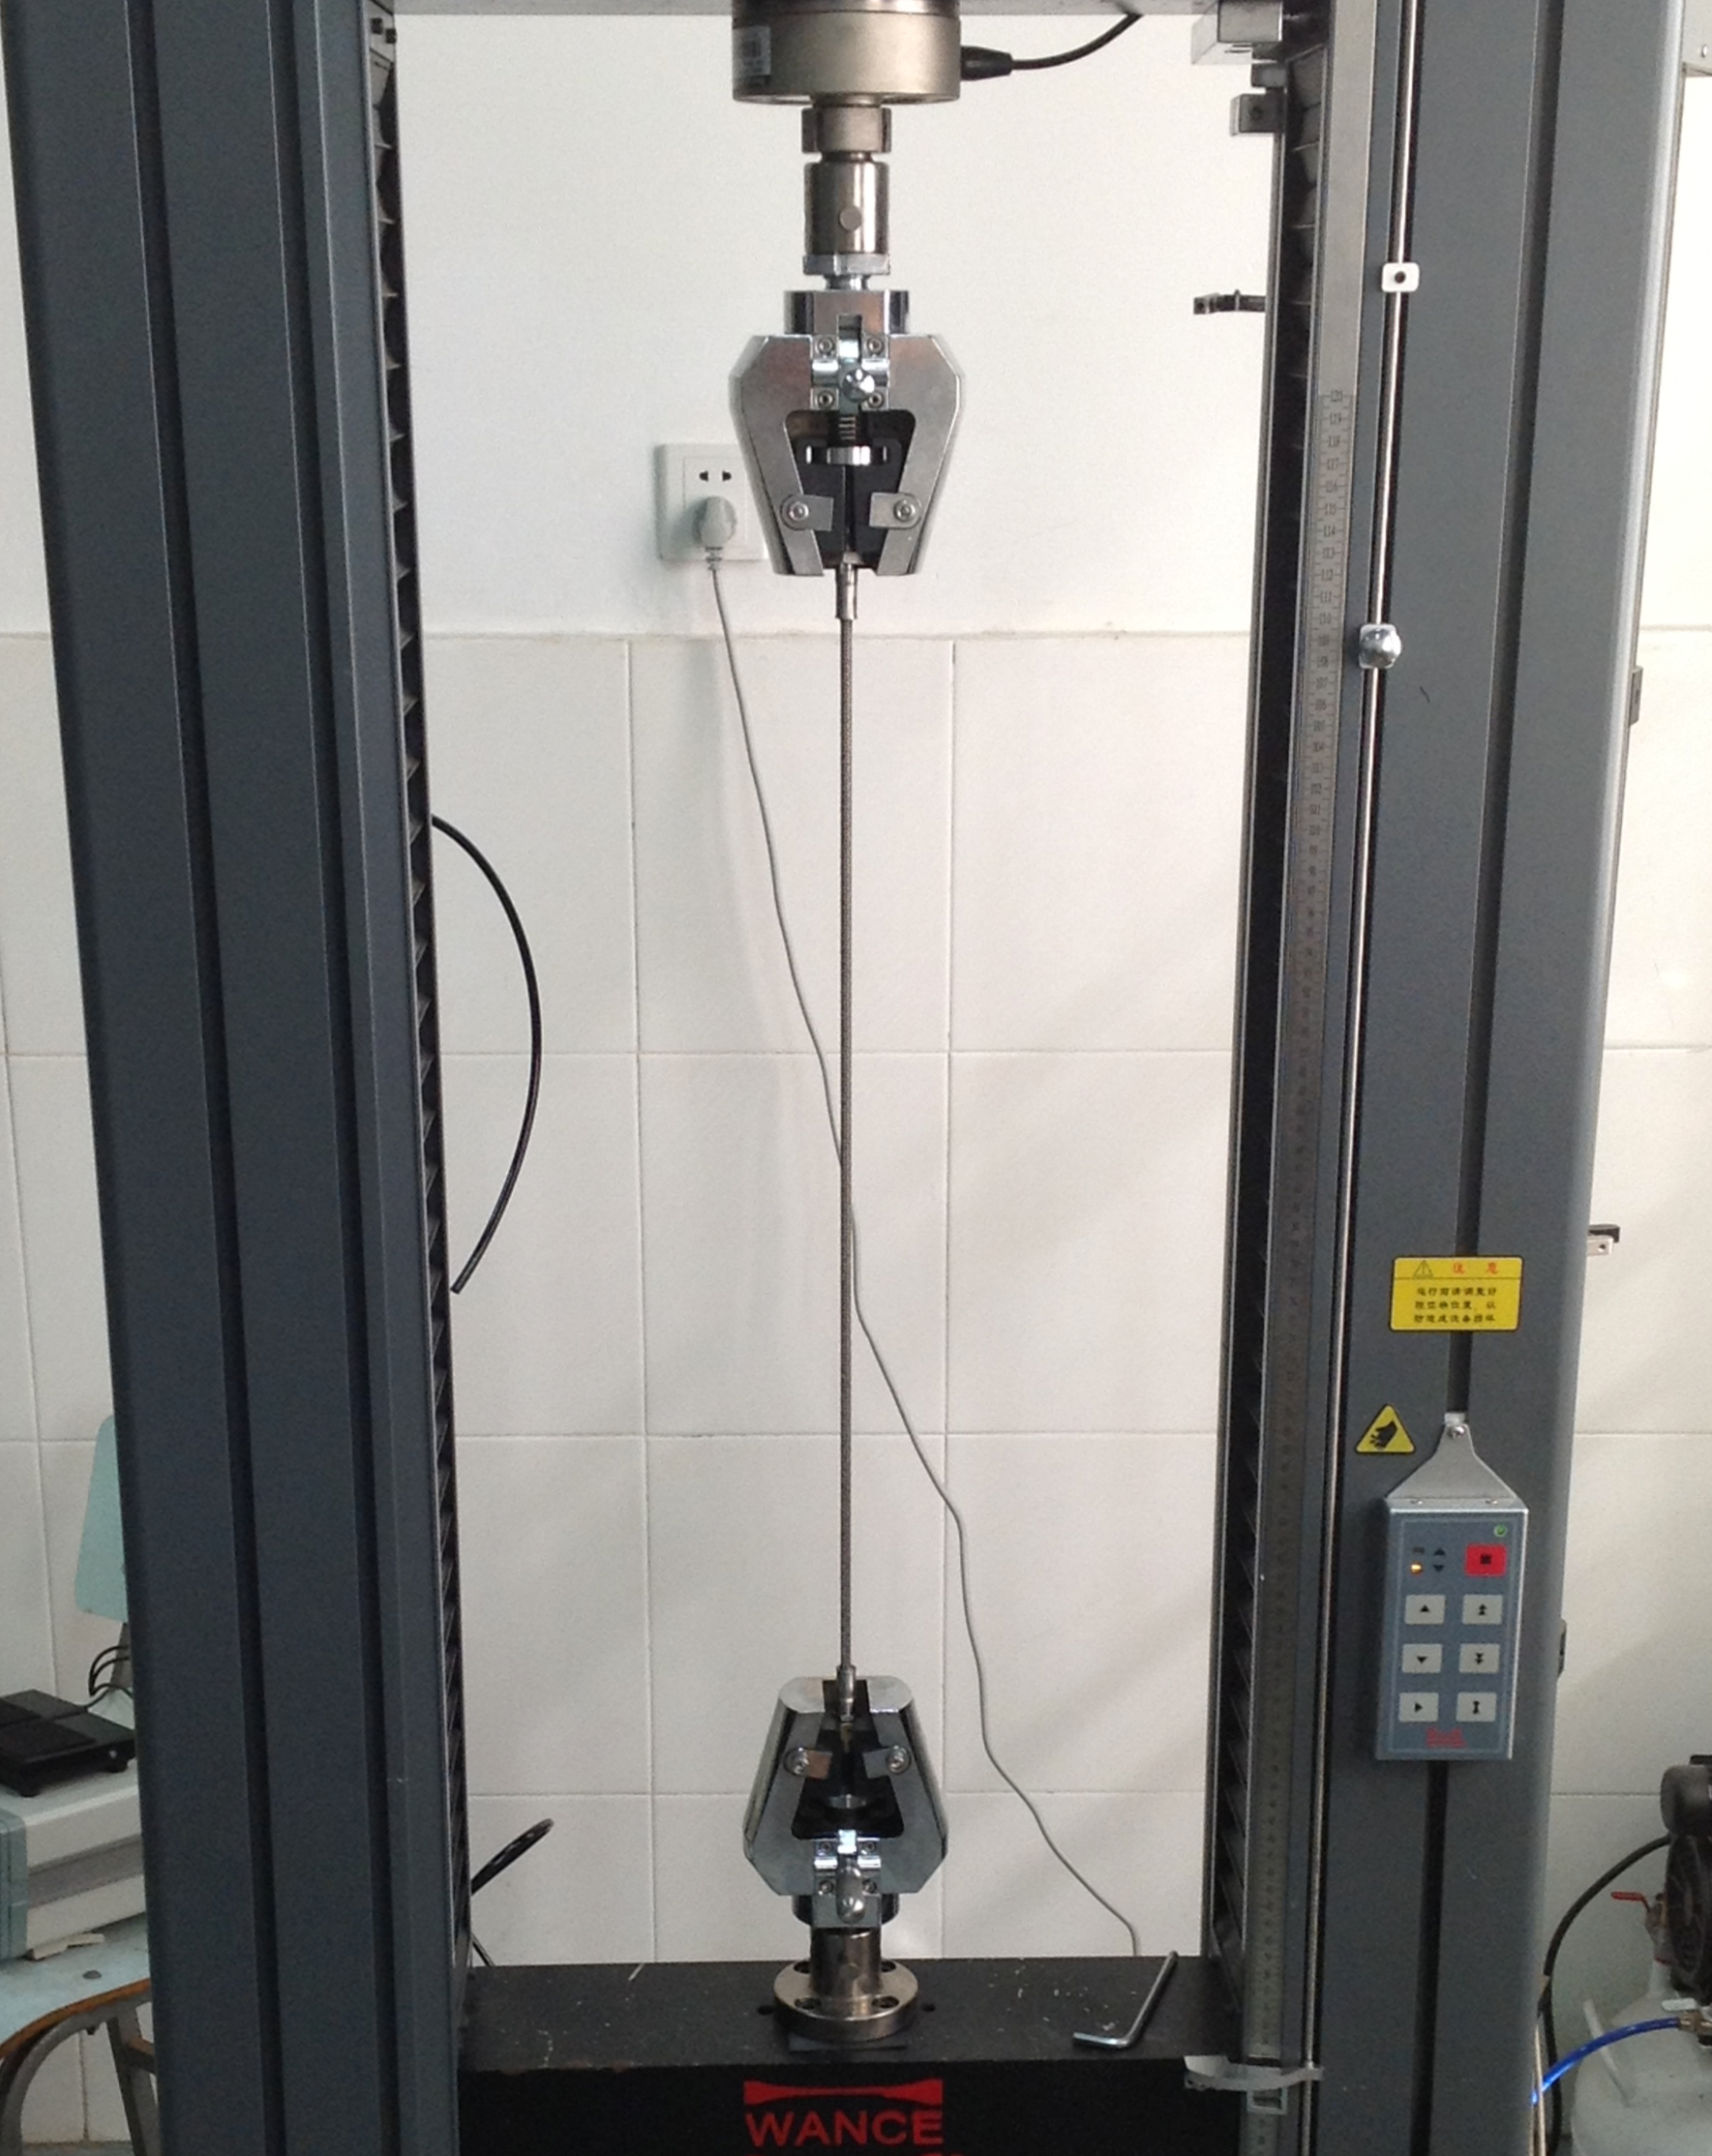
\includegraphics[height=0.3\textheight]{figure/experiment/tensile}
%		\label{experiment-1}
%	}
%	\hspace{1.2cm}
%	\subfigure{
%		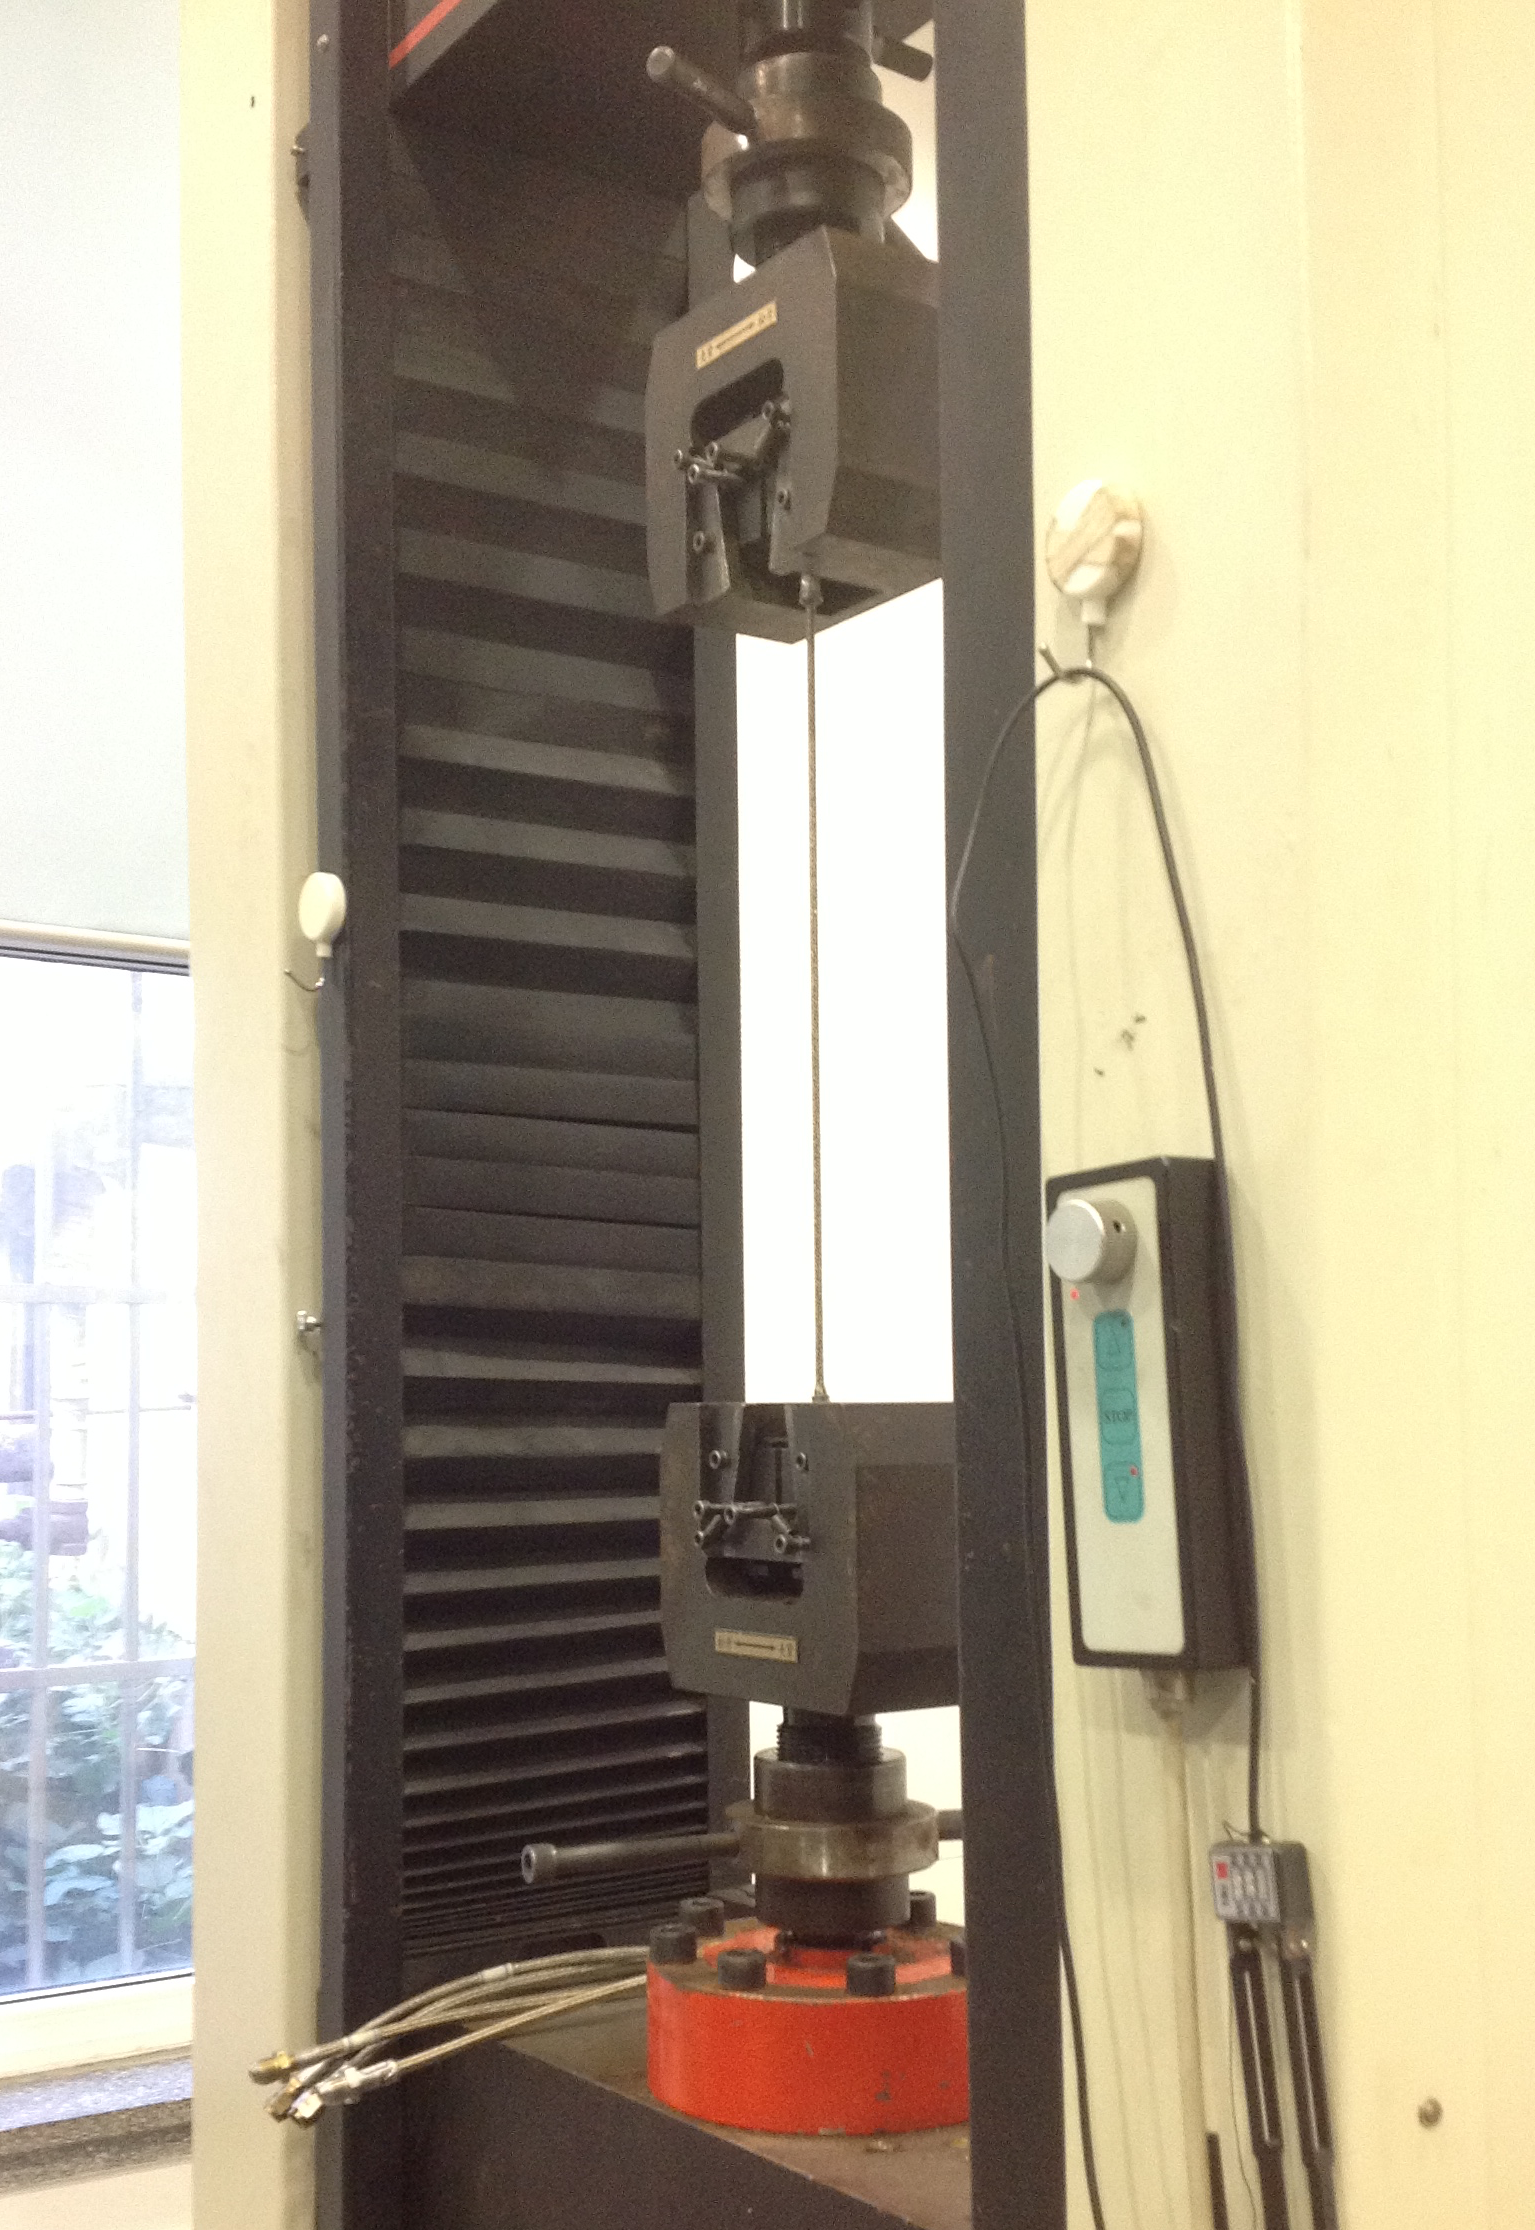
\includegraphics[height=0.3\textheight]{figure/experiment/experiment-1}
%		\label{experiment-2}
%	}

	\fcaption{力学万能试验机}{Universal tensile machine}  
	\label{fig:experiment}
\end{figure}



\section{实验步骤}

\begin{compactenum}
	\item 将软管安装至万能试验机,一般软管组件的接头较为粗大,需要通过公装连接试验机夹具;
	\item 开始拉伸实验,加载速度不能超过10mm/min;
	\item 工程应变每增加0.05,至少记录一组数据,
	\begin{compactitem}
		\item 支座反力和软骨啊伸长量有试验机系统记录;
		\item 用拓印法记录编织角,至少3个染色区域,分别拓印记录;
		\item 记录染色区域的管径变化;
		\item 记录数据时拉伸的过程不会停止,必须短时间内测量记录各组数据,保证数据具有可比性。
	\end{compactitem}
	\item 试件破坏,实验结束。
\end{compactenum}





\section{第一次拉伸实验}
\subsection{试件参数}
 实验试件如图\ref{fig:experiment-1-specimen}所示。试件分别编号为芯棒1、芯棒2、芯棒3,芯棒4,共4组。
 “芯棒”代表试件制备的方法:编织机直接在将钢丝编织在芯棒上,然后抽出芯棒,仅保留编织层连接接头工装。
由于抽拔芯棒的过程,各组试件的编织角大幅小于平衡角。



\begin{figure}[!htb]
	\centering
	\subfigure[]{
		\includegraphics[width=0.4\textwidth]{figure/experiment/E1/specimen/E1-1}}
	\hspace{1cm}
	\subfigure[]{
		\includegraphics[width=0.4\textwidth]{figure/experiment/E1/specimen/E1-2}}
	
	\subfigure[]{
		\includegraphics[width=0.4\textwidth]{figure/experiment/E1/specimen/E1-3}}
	\hspace{1cm}
	\subfigure[]{
		\includegraphics[width=0.4\textwidth]{figure/experiment/E1/specimen/E1-4}}
	\fcaption{第一次拉伸实验试件}{characteristics of specimen in 1st traction experiment}  
	\label{fig:experiment-1-specimen}
\end{figure}

\begin{table}[!htb]
	\centering
	\tcaption{第一次拉伸实验试件}{Hose Specimen of the traction experiment}
	\label{tab:hose-specimen}
	\begin{tabular*}{0.8\textwidth}{@{\extracolsep{\fill}}>{\hspace{0.5cm}}cccc}
		\toprule
		                  &     编织层-1     &     编织层-2     &     编织层-3     \\ \midrule
		外径(mm)            &     7.60      &     7.59      &     7.60      \\
		内径 (mm)           &     6.80      &     6.77      &     6.81      \\
		长度 (mm)           &     320.0     &     321.0     &     320.5     \\
		编织角 (\textdegree) &     42.1      &     41.9      &      43       \\
		股数$ \times $根数    & 24$ \times $6 & 24$ \times $6 & 24$ \times $6 \\
		钢丝直径(mm)          &      0.2      &      0.2      &      0.2      \\ \bottomrule
	\end{tabular*} 
\end{table}













\subsection{力位移曲线}
实验结果如图\ref{fig:experiment-results-1}所示,图为拉伸支座反力和拉伸量之间的关系,下文统一称之为“力-位移曲线”。
第一次拉伸实验共准备四组试件,对其中3组进行了拉伸实验。试件Hose-1拉伸至接头钢丝断裂破坏,Hose-2、Hose-3并未拉伸至破坏。观察三组拉伸实验的力-位移曲线结果,Hose-2与Hose-1的前段几乎完全重合;三组试件的结果趋势,大小一致,可见试件的质量、力学性质稳定,实验结果可信;实验结果中体现的编织层在应变较大时变现出来的高度的非线性,与\ha 文献中的结果比较类似。



\begin{figure}[!htb]
	\centering
	\includegraphics[width=0.6\textwidth]{figure/experiment/E1/Graph01}
	
	\subfigure[]{
		\includegraphics[width=0.3\linewidth]{figure/experiment/E1/Graph03}}
	\subfigure[]{
		\includegraphics[width=0.3\linewidth]{figure/experiment/E1/Graph04}}
	\subfigure[]{
		\includegraphics[width=0.3\linewidth]{figure/experiment/E1/Graph05}}
	
	\fcaption{第一次拉伸实验力位移曲线}{load displacement curve of 1st experiment}  
	\label{fig:experiment-results-1}
\end{figure}



\subsection{破坏形式}

编织层试件拉伸过程中,接头处会发生颈缩的现象,最终也在接头处发生断裂破坏,如\ref{fig:experiment-1-fail}所示。



\begin{figure}[!htb]
	\centering
	\subfigure{
		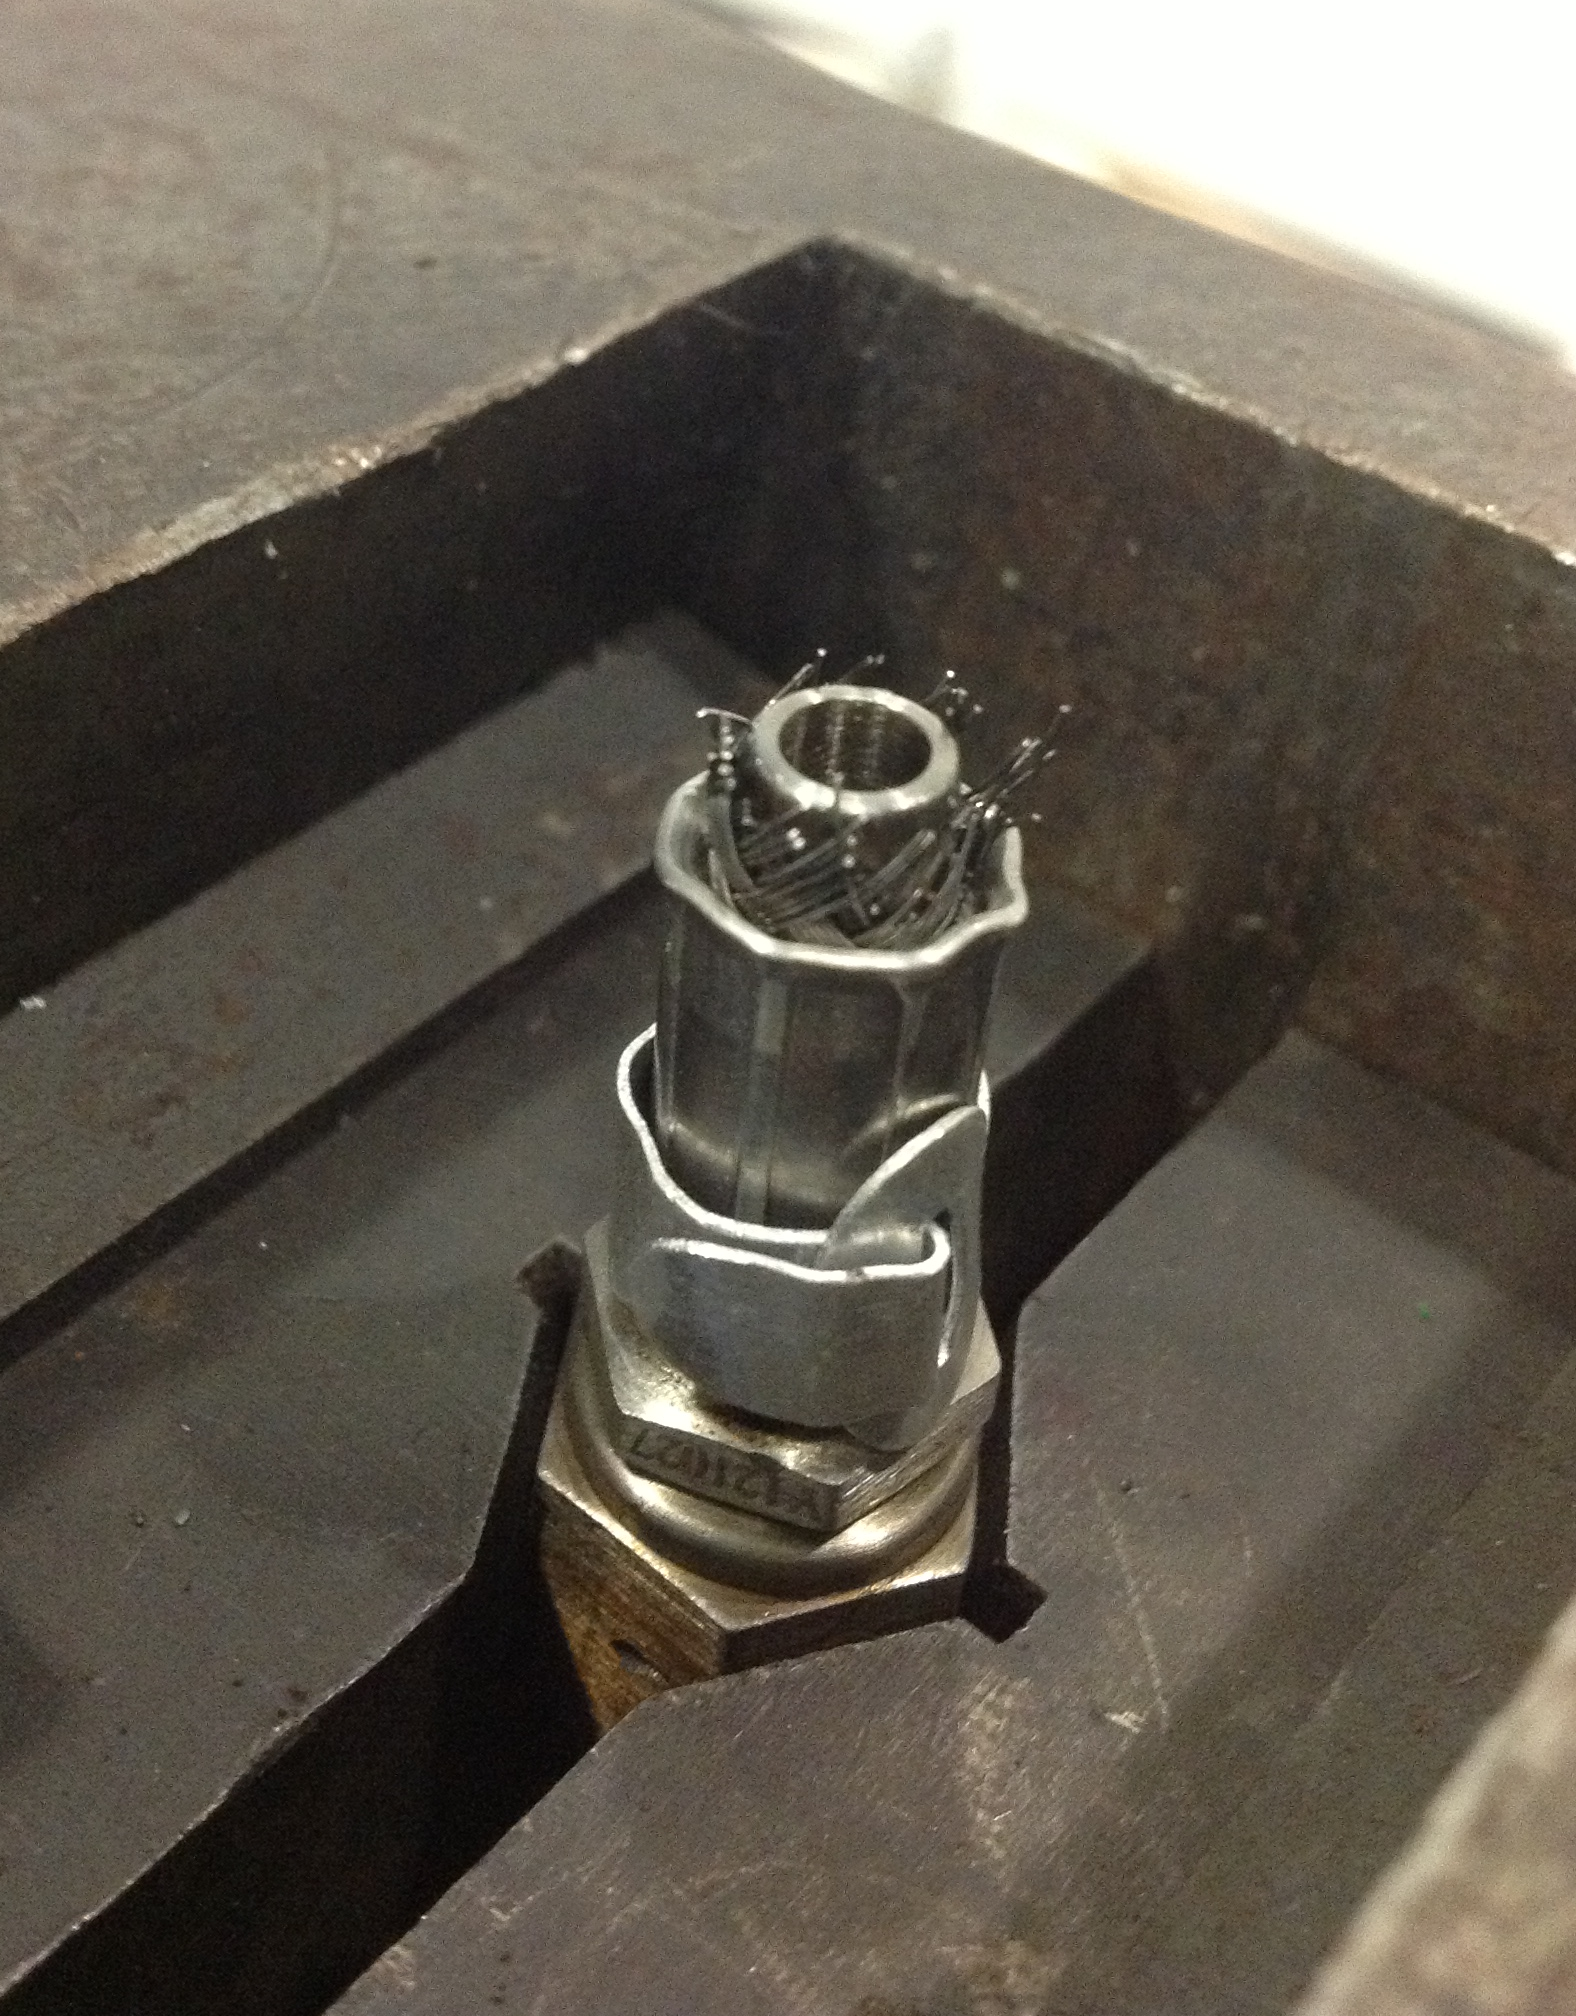
\includegraphics[height=0.18\textheight]{figure/experiment/E1/failure-1}}
	\hspace{0.3cm}
	\subfigure{
	\includegraphics[height=0.18\textheight]{figure/experiment/E1/failure-2}}
	\hspace{0.3cm}
	\subfigure{
		\includegraphics[height=0.18\textheight]{figure/experiment/E1/necking}}
	\fcaption{破坏形式}{Damage form of specimen in 1st experiment}
	\label{fig:experiment-1-fail}
\end{figure}









\section{第二次拉伸实验}

根据第一次拉伸实验结果,软管组件拉伸最大荷载很难超过1t,因而第二次拉伸实验采用了量程更小的5t万能试验机,可以更准确的记录软管组件拉伸的力位移曲线。

\subsection{试件参数}
第二次拉伸实验的软管试件包含了PTFE材质的内管,各项参数与普通使用的软管基本一致。同时实验进行了PTFE内管的拉伸实验,因为不同配方,不同烧制工艺会影响到PTFE材料的力学性能。
 ,实验试件共4组,其中两组PTFE内管,两组为软管组件。表\ref{tab:hose-specimen-II}以及图\ref{fig:PTFE-braid-tube-1}为带编织层的两组试件。
\begin{table}[!htb]
	\centering
	\tcaption{第二次拉伸实实验试件参数}{characteristics of  specimen in 2nd traction experiment}
	\label{tab:hose-specimen-II}
	\begin{tabular*}{0.8\textwidth}{@{\extracolsep{\fill}}>{\hspace{0.5cm}}ccc}
		\toprule
		&     软管组件-1     &     软管组件-2     \\ \midrule
		软管形式& 编织层+PTFE内管&编织层+PTFE内管\\
		编织层外径(mm)            &     7.60      &     7.59      \\
		内管内径 (mm)           &     4.99      &     5.01      \\
		软管长度 (mm)           &     420.0     &     421.5     \\
		编织角 (\textdegree) &     52.1      &     53      \\
		股数$ \times $根数    & 24$ \times $6 & 24$ \times $6 \\
		钢丝直径(mm)          &      0.2      &      0.2      \\ \bottomrule
	\end{tabular*} 
\end{table}


\begin{figure}[!htp]
	\centering
	\subfigure[]{
		\includegraphics[height=0.15\textheight]{figure/experiment/E2/PTFE-braid-tube-1}
		\label{fig:PTFE-braid-tube-1}
	}
	\hspace{0.5cm}
	\subfigure[]{
		\includegraphics[height=0.15\textheight]{figure/experiment/E2/PTFE-braid-tube-2}
		\label{fig:PTFE-braid-tube-2}
	}
	\fcaption{第二次拉伸实验试件}{Hose Specimen in 2nd traction experiment}
	\label{fig:tesile-experiment-II}
\end{figure}








\subsection{力位移曲线}
实验结果力位移曲线如图\ref{fig:experiment-2}所示,

\begin{figure}[!htb]
	\centering
	\includegraphics[width=0.6\textwidth]{figure/experiment/E2/Graph01}
	
	\subfigure[]{
			\includegraphics[width=0.37\textwidth]{figure/experiment/E2/Graph02}
			}
	\subfigure[]{
			\includegraphics[width=0.37\textwidth]{figure/experiment/E2/Graph03}
		}
	\fcaption{第二次拉伸实验力位移曲线}{load displacement curve of 2nd experiment}  
	\label{fig:experiment-2}
\end{figure}


\subsection{破坏形式}



第二组带内管的试件的破坏形式如图\ref{fig:failure-experiment-ii}所示,编织层仍然在接头处钢丝断裂破坏。

\begin{figure}[!htp]
\centering
\subfigure{
\includegraphics[height=0.21\textheight]{figure/experiment/E2/fail-1}
\label{fig:fail-1}
}
\hspace{1cm}
\subfigure{
\includegraphics[height=0.21\textheight]{figure/experiment/E2/fail-2}
\label{fig:fail-2}
}
\fcaption{破坏形式}{Damage form of specimen in 2nd experiment}
\label{fig:failure-experiment-ii}
\end{figure}


\subsection{PTFE内管拉伸试件参数及结果}

PTFE内管参数如表\ref{tab:hose-specimen-II-22}所示。由于PTFE断裂伸长率在$ 100\% $以上\cite{zhuyouliang2006},试件很难拉伸至断裂。
\begin{table}[!htb]
	\centering
	\tcaption{PTFE内管试件参数}{characteristics of inner PTFE tube Specimen}
	\label{tab:hose-specimen-II-22}
	\begin{tabular*}{0.8\textwidth}{@{\extracolsep{\fill}}>{\hspace{0.5cm}}ccc}
		\toprule
		&      内管-1     &     内管-2     \\ \midrule
		软管形式& PTFE内管&PTFE内管\\
		外径(mm)            &     7.01      &     6.99      \\
		内径 (mm)           &     5.00      &     5.01      \\
		长度 (mm)           &     420.0     &     423     \\ \bottomrule
	\end{tabular*} 
\end{table}


\begin{figure}[!htb]
	\centering
	\subfigure[]{
		\includegraphics[height=0.13\textheight]{figure/experiment/E2/PTFE-inner-tube-1}
		\label{fig:PTFE-inner-tube-1}
	}
	\hspace{1cm}
	\subfigure[]{
		\includegraphics[height=0.13\textheight]{figure/experiment/E2/PTFE-inner-tube-2}
		\label{fig:PTFE-inner-tube-2}
	}
	\fcaption{PTFE内管试件拉伸力位移曲线}{load displacement curve of inner PTFE tube Specimen traction}
	\label{fig:tesile-experiment-II}
\end{figure}


\begin{figure}[!htb]
\centering
\subfigure[]{
\includegraphics[height=0.2\textheight]{figure/experiment/E2/PTFE}
\label{fig:PTFE-2}
}
\hspace{0.5cm}
\subfigure[]{
\includegraphics[height=0.2\textheight]{figure/experiment/E2/PTFE-2}
\label{fig:PTFE}
}
\fcaption{PTFE内管拉伸实验结果}{PTFE inner tube traction results}
\label{fig:PTFE-traction}
\end{figure}


实验同时也确定了PTFE内管的力学性能,拉伸的力位移曲线如图\ref{fig:PTFE-traction},对比同口径带编织层的软管(图\ref{fig:PTFE}),可以观察到软管拉伸量较小,总体应变量小于0.06时,拉力主要由软管组件的内管承担。



\newpage
\section{第三次拉伸实验}
\subsection{试件参数}
  第三次拉伸实验对两个规格的PTFE软管组件进行了拉伸,分别类8mm口径和18mm口径。
  
  实验试件共分分为四组,8mm口径、18mm口径各两组,每组按不同编织密度制作试件分别为65\%、70\%、80\%、90\%,分别标记为BD-65、BD-70、BD-80、BD-90,BD代表编织密度(Braid Density)。各试件具体几何参数如表\ref{tab:hose-specimen-III-1}所示。其中编织密度较低的试件,如BD-65、BD-70,按照正常流程还需要增加外套层保证结构稳定;本实验为了保证可以测量编织层编织角的变化,没有增加外套层。
  
  
%  试件参数
  
  \begin{table}[!htb]
  	\centering
  	\tcaption{ 第三次拉伸实验试件参数}{characteristics of  specimen in 3rd traction experiment}
  	\label{tab:hose-specimen-III-1}
  	\begin{tabular*}{0.8\textwidth}{@{\extracolsep{\fill}}>{\hspace{0.5cm}}ccccc}
  		\toprule
  		\textbf{第一组}&     BD-65     &     BD-70     &     BD-80     &     BD-90     \\ \midrule
  		编织层外径(mm)  & 26.8         &     24.63     &     22.06     &     19.22       \\
  		软管长度 (mm)    & 320          &      323      &      322      &      325       \\
  		编织角 (\textdegree)   & 46.76 &     48.22     &     47.41     &     53.56     \\
  		股数$ \times $根数          & 24$ \times $6 & 24$ \times $6 & 24$ \times $6 & 24$ \times $6 \\
  		钢丝直径(mm)                &      0.2      &      0.2      &      0.2      &      0.2      \\ \bottomrule
  	\end{tabular*} 
  \end{table}
  
  \begin{table}[!htb]
  	\centering

  	\begin{tabular*}{0.8\textwidth}{@{\extracolsep{\fill}}>{\hspace{0.5cm}}ccccc}
  		\toprule
  		\textbf{第二组}          &     BD-65     &     BD-70     &     BD-80     &     BD-90     \\ \midrule
  		编织层外径(mm)  & 27.23      &     26.23     &     20.48     &     22.8        \\
  		软管长度(mm)    & 319       &      322      &      322      &      321        \\
  		编织角(\textdegree)& 45.75 &     50.00     &     48.42     &     51.08      \\
  		股数$ \times $根数        & 24$ \times $6 & 24$ \times $6 & 24$ \times $6 & 24$ \times $6 \\
  		钢丝直径(mm)              &      0.2      &      0.2      &      0.2      &      0.2      \\ \bottomrule
  	\end{tabular*} 
  \end{table}
  
  \begin{table}[!htb]
  	\centering
  	\begin{tabular*}{0.8\textwidth}{@{\extracolsep{\fill}}>{\hspace{0.5cm}}ccccc}
  		\toprule
  		\textbf{第三组}       &     BD-65     &     BD-70     &     BD-80     &     BD-90     \\ \midrule
  		编织层外径(mm)  10.16   &     10.28     &     9.75      &     9.91      &     9.66      \\
  		软管长度(mm)    318    &      319      &      319      &      318      &      323      \\
  		编织角(\textdegree)32 &     43.66     &     46.62     &     47.82     &     51.03     \\
  		股数$ \times $根数     & 24$ \times $6 & 24$ \times $6 & 24$ \times $6 & 24$ \times $6 \\
  		钢丝直径(mm)           &      0.2      &      0.2      &      0.2      &      0.2      \\ \bottomrule
  	\end{tabular*} 
  \end{table}  

  \begin{table}[!htb]
  	\centering
  	\begin{tabular*}{0.8\textwidth}{@{\extracolsep{\fill}}>{\hspace{0.5cm}}ccccc}
  		\toprule
  		\textbf{第四组}          &     BD-65     &     BD-70     &     BD-80     &     BD-90     \\ \midrule
  		编织层外径(mm)  & 10.23      &     10.06     &      9.6      &      8.5        \\
  		软管长度(mm)    & 322       &      325      &      327      &      326        \\
  		编织角(\textdegree)& 42.58 &     44.96     &     49.90     &     50.24       \\
  		股数$ \times $根数        & 24$ \times $6 & 24$ \times $6 & 24$ \times $6 & 24$ \times $6 \\
  		钢丝直径(mm)              &      0.2      &      0.2      &      0.2      &      0.2      \\ \bottomrule
  	\end{tabular*} 
  \end{table}


\begin{figure*}
\centering
\includegraphics[height=0.25\textheight]{figure/experiment/18mm-hose-specimen}
\fcaption{实验试件编织密度对比}{ comparation of hose specimen with different braid densisty}
\label{fig:Slice1}
\end{figure*}


\subsection{实验结果}
本研究拉伸实验共进行三次,前两次采用的是摄影法,实验效果并不令人满意。只采用了相对较为准确的初始测量角,因其拍摄条件可控;第三次采用拓印法,记录的数据可靠可信,实验中不仅记录了初始编织角,还记录了过程中的编织角变化。

\begin{table}[!htb]
	\centering
	\tcaption{各组实验编织角测量方法}{Braid Angel Measuring Method of Hoses}
	\label{tab:hose-specimen-II-2}
	\begin{tabular}{@{\extracolsep{\fill}}>{\hspace{0.5cm}}ccccc}
		\toprule
		& 编织角测量方法 &   起始编织角    &  过程编织角变化   &   测量准确性    \\ \midrule
		拉伸实验 &   摄影法   & \checkmark &            &  \\
		拉伸实验 &   摄影法   & \checkmark &            &  \\
		拉伸实验 &   拓印法   & \checkmark & \checkmark & \checkmark \\ \bottomrule
	\end{tabular} 
\end{table}

\newpage

\subsubsection{第一组试件}

第一组试件的位移曲线如图\ref{fig:E3-g1}所示, 其中编织密度较低的两组试件存在力位移曲线陡增的情况。这是由于编织密度低的试件编织层较为松散,没有与内管紧密贴合,拉伸时前段由PTFE内管受力,编织层受力时,力位移曲线就发生了陡增的情况。

\begin{figure}[!htb]
	\centering
	
	\subfigure{
		\includegraphics[height=0.35\textheight]{figure/experiment/E3-G1/Graph01}}
	\subfigure{
		\includegraphics[height=0.4\textheight]{figure/experiment/E3-G1/Graph02}}
	
	\fcaption{第一组软管组件力位移曲线}{Group.1 Hose Assembly load displacement curve}   
	\label{fig:E3-g1}
\end{figure}

\subsubsection{第二组试件}

第一组试件的位移曲线如图\ref{fig:E3-g2}所示,
\begin{figure}[!htb]
	\centering
	
	\subfigure{
		\includegraphics[height=0.35\textheight]{figure/experiment/E3-G2/Graph01}}
	\subfigure{
		\includegraphics[height=0.4\textheight]{figure/experiment/E3-G2/Graph02}}
	
	\fcaption{第二组软管组件力位移曲线}{Group.2 Hose Assembly load displacement curve}  
	\label{fig:E3-g2}
\end{figure}




\subsubsection{第三组试件}

第三组试件的位移曲线如图\ref{fig:E3-g3}所示,
\begin{figure}[!htb]
	\centering
	
	\subfigure{
		\includegraphics[height=0.35\textheight]{figure/experiment/E3-G3/Graph01}}
	\subfigure{
		\includegraphics[height=0.4\textheight]{figure/experiment/E3-G3/Graph02}}
	
	\fcaption{第三组软管组件力位移曲线}{Group.3 Hose Assembly load displacement curve}  
	\label{fig:E3-g3}
\end{figure}

\subsubsection{第四组试件}

第四组试件的位移曲线如图\ref{fig:E3-g4}所示,
\begin{figure}[!htb]
	\centering
	
	\subfigure{
		\includegraphics[height=0.35\textheight]{figure/experiment/E3-G4/Graph01}}
	\subfigure{
		\includegraphics[height=0.4\textheight]{figure/experiment/E3-G4/Graph02}}
	
	\fcaption{第四组软管组件力位移曲线}{Group.4 Hose Assembly load displacement curve}  
\label{fig:E3-g4}
\end{figure}

\subsection{破坏形式}

各组试件接头处发生脱头的现象,如图\ref{fig:fail-experiment-III},因此软管拉伸失效时,编织层钢丝有别与之前的两次实验,均为发生断裂如图\ref{fig:E3-hose-fail}所示。

\begin{figure}[!htb]
	\centering
	\subfigure{
		\includegraphics[height=0.25\textheight]{figure/experiment/E3-G3/Specimen/fail-2}
		\label{fig:fail-2}
	}
	\hspace{1cm}
	\subfigure{
		\includegraphics[height=0.25\textheight]{figure/experiment/E3-G3/Specimen/fail}
		\label{fig:fail}
	}
	\fcaption{试件破坏形式}{ Damage forms of hose traction}
	\label{fig:fail-experiment-III}
\end{figure}


\begin{figure}[!htb]
	\centering
	\subfigure{
		\includegraphics[height=0.18\textheight]{figure/experiment/E3-G3/Specimen/fail-g1}
		\label{fig:fail-g1}
	}
	\hspace{0.5cm}
	\subfigure{
		\includegraphics[height=0.18\textheight]{figure/experiment/E3-G3/Specimen/fail-g2}
		\label{fig:fail-g2}
	}
	\hspace{0.5cm}
	\subfigure{
		\includegraphics[height=0.18\textheight]{figure/experiment/E3-G3/Specimen/fail-g3}
		\label{fig:fail}
	}
	\hspace{0.5cm}
	\subfigure{
		\includegraphics[height=0.18\textheight]{figure/experiment/E3-G3/Specimen/fail-g4}
		\label{fig:fail-g4}
	}
	\fcaption{第三组试件破坏形式}{ Damage forms of groups of hoses}
	\label{fig:E3-hose-fail}
\end{figure}



\newpage

\subsection{编织角变化}
如图\ref{fig:braid-angle-variation}所示,为各组试件中BD-90软管的编织角在拉伸中的变化。

\begin{figure}[!htb]
\centering
\subfigure[第一组]{
\includegraphics[height=0.2\textheight]{figure/experiment/g1-90}
\label{fig:g1-90}
}
\subfigure[第二组]{
\includegraphics[height=0.2\textheight]{figure/experiment/g2-90}
\label{fig:g2-90}
}
\subfigure[第三组]{
\includegraphics[height=0.2\textheight]{figure/experiment/g3-90}
\label{fig:g3-90}
}
\subfigure[第四组]{
\includegraphics[height=0.2\textheight]{figure/experiment/g4-90}
\label{fig:g4-90}
}
\fcaption{编织角变化}{Braid Angle Variation}
\label{fig:braid-angle-variation}
\end{figure}


可能由于编织角采样频率的限制,不同编织密度与编织角的变化趋势间,没有体现出相关性。编织角基本维持线性减小的趋势。

\begin{figure*}[!htb]
\centering
%\subfigure{
%\includegraphics[width=0.3\textwidth]{figure/experiment/braid-angle/g1-65}
%\label{fig:g1-65}
%}
\subfigure{
\includegraphics[width=0.3\textwidth]{figure/experiment/braid-angle/g1-70}
\label{fig:g1-70}
}
\subfigure{
\includegraphics[width=0.3\textwidth]{figure/experiment/braid-angle/g1-80}
\label{fig:g1-80}
}
\subfigure{
\includegraphics[width=0.3\textwidth]{figure/experiment/braid-angle/g1-90}
\label{fig:g1-90-2}
}
\fcaption{不同编织密度与编织角的变化关系}{relation between braid density and braid angle variaion}
\label{fig:g1-braid-angle}
\end{figure*}




\newpage



\section{实验结果分析}

本研究拉伸实验得到了几组试件拉伸的力位移曲线,结果与
\ha 试件的拉伸结果一致,都体现出了软管组件编织层受拉时的非线性力学行为。






\subsection{编织角不锁定}

第三次拉伸实验所记录的拉伸过程中编织角变化,可以比较明显的观察到,力位移曲线在发生非线性的变化是,编织角是保持变化的。如图\ref{fig:angle-conclusion}所示,该组实验中对编织角的采样较为密集,可以清楚的看到编织角保持着减小的趋势;可见编织角不会发生锁定。根据\ref{eq:lockalpha}计算该试件的$ \alpha_{lock} $为$ 38.43\textdegree $,而实验中试件的编织角持续较小,达到$ 32.16\textdegree $。

\begin{figure}[!htb]
	\centering
	\subfigure[]{
		\includegraphics[height=0.35\textheight]{figure/experiment/g1-90}
		\label{fig:g1-90}
	}
	\fcaption{编织角变化}{Braid Angle Variation}
	\label{fig:angle-conclusion}
\end{figure}

观察实验采集的各组试件编织角的数据,发现编织角基本上呈线性变化, 对其进行线性拟合,各组编织角拟合的趋势线均能较好的吻合实验数据结果。




\subsection{金属纤维生塑性应变}




在3次试验中挑选典型试验结果进行比对,如表\ref{tab:hose-comparation}所示,拉伸的力位移曲线如图\ref{fig:hose-comparation}所示。第一次、第二次拉伸实验中的试件的破坏形式均为接头处钢丝断裂。因此可以断定,接头处得钢丝一定发生了塑性变形,但是其他区域的金属纤维是否发生塑性变形需要进一步的分析。



\begin{table}[!htb]
	\centering
	\tcaption{代表性试件破坏形式}{Hose Specimen of the traction experiment}
	\label{tab:hose-comparation}
	\begin{tabular}{@{\extracolsep{\fill}}>{\hspace{0.5cm}}cccc}
		\toprule
		实验组别 & 试件编号& 软管组件形式& 破坏形式\\\midrule
		实验I& 芯棒1& 编织层& 接头钢丝断裂\\
		实验II& 软管组件2& 编织层+内管& 接头钢丝断裂\\
		实验III& 第一组-BD-80& 编织层+内管& 接头脱头\\\bottomrule
	\end{tabular} 
\end{table}  


\begin{figure}[!htb]
	\centering
	\subfigure[]{
		\includegraphics[height=0.22\textheight]{figure/chap2/plasiticity-3}
		\label{fig:hose-comparation-1}}
	\subfigure[]{
		\includegraphics[height=0.22\textheight]{figure/chap2/plasiticity-2}
		\label{fig:hose-comparation-2}}
	\subfigure[]{
		\includegraphics[height=0.22\textheight]{figure/chap2/plasiticity-1}
		\label{fig:hose-comparation-3}}
	\fcaption{各组力位移曲线趋势对比对比}{contrast of trends of experimental results}
	\label{fig:hose-comparation}
\end{figure}




由于编织层采用的钢丝断裂伸长率仅为约$ 2\% $

图\ref{fig:hose-comparation-1}中,试件的力位移曲线没有出现类似\ha 试件的拐点,实验中观察不到钢丝发生塑性应变;断裂时现象类似脆断。

图\ref{fig:hose-comparation-2}中,力位移曲线轻微偏离非线性增长的趋势,直到最后组件发生脆断。

事实上,断裂后的软管组件试件仍能大致恢复拉伸前的形态,结合图\ref{fig:hose-comparation-1}、图\ref{fig:hose-comparation-2},本研究认为:拉伸实验时,仅有接头附近发生颈缩的区域的金属纤维发生塑像变形,力位移曲线仅在软管组件整体断裂之前的一小段轻微偏离非线性的趋势。



观察图\ref{fig:hose-comparation-3},试件的力位移曲线较大偏离了非线性增长的趋势。而偏离段的实验过程中,可以发现软管组件接头扣压逐渐松脱。可以认为,若力位移曲线较大偏离原有的非线性趋势,一般是由于接头脱头导致。

综合分析这些实验现象和实验数据,本研究认为:编织层采用断裂伸长率较小的钢丝时,钢丝轻微的塑性变形不会导致编织层结构在拉伸时,出现刚度降低的拐点。拐点的出现更有可能的原因是:接头扣压随着软管内管管壁在拉伸过程中逐渐变薄而逐渐失效,接头中的钢丝逐渐从扣押的约束中释放导致刚度降低;钢丝完全释放则软管发生脱头现象,不完全释放则在钢丝到达极限伸长量时断裂。



\section{小~结}
本章主要介绍了本研究的实验内容。本研究的实验实验主要包括3次拉伸实验。

三次拉伸实验的区别主要在试件:
\begin{compactitem}
	\item 第一次拉伸实验的试件不包含内管,仅有编织层;
	\item 第二次拉伸实验试件包含内管,并测试了内管的力学性质;
	\item 第三次拉伸实验对比了不同编织密度试件的拉伸曲线,不同编著密度区别主要在编织角度。
\end{compactitem}

本章还提出了准确且简便测量编织角的方法,属于本文首创,这对于软管编织层的研究至关重要,因为编织角度对纤维编织加强层的本构影响非常之大。

此外,本章还针对\ha 拉伸实验中提出的两个假设,结合本实验的结果进行了分析,认为:
\begin{compactitem}
	\item 金属纤维编织加强层只在小范围内产生塑性变形,其效果相对接头失效的影响要小得多;
	\item 编织角不发生锁定,且在拉伸时,一直呈线性减小的趋势。
\end{compactitem}